% generated by experiments/build_paper_assets.py -- do not edit by hand
\begin{figure}[t]
\centering
\resizebox{\linewidth}{!}{%
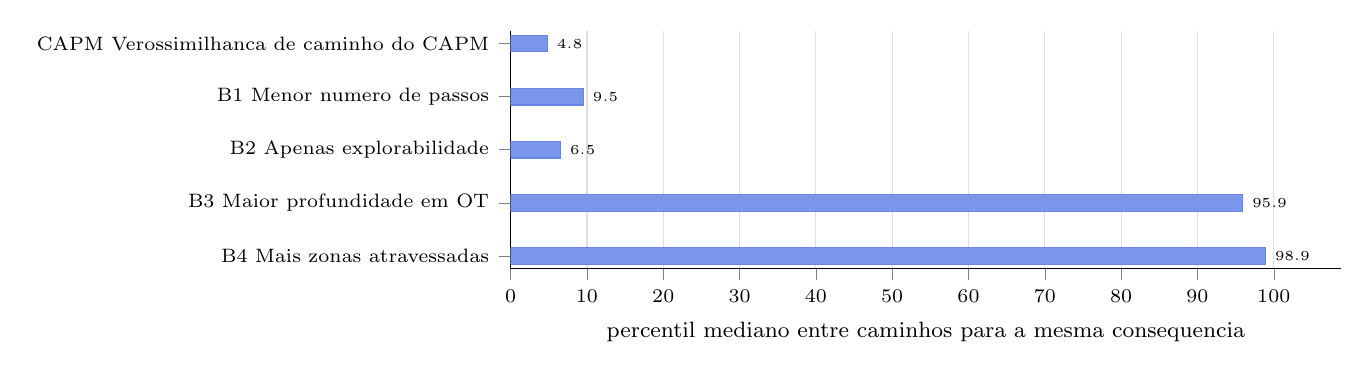
\begin{tikzpicture}
\begin{axis}[
    xbar, width=\linewidth, height=4.6cm,
    xlabel={percentil mediano entre caminhos para a mesma consequencia},
    xmin=0, enlarge y limits=0.06,
    ytick={0,1,2,3,4}, yticklabels={{CAPM Verossimilhanca de caminho do CAPM},{B1 Menor numero de passos},{B2 Apenas explorabilidade},{B3 Maior profundidade em OT},{B4 Mais zonas atravessadas}},
    y dir=reverse, ticklabel style={font=\scriptsize},
    label style={font=\footnotesize},
    nodes near coords, nodes near coords style={font=\tiny},
    every node near coord/.append style={/pgf/number format/fixed,
        /pgf/number format/precision=3},
    xmajorgrids, grid style={gray!25}, axis lines*=left,
    bar width=6pt, tick align=outside,
]
\addplot[fill=RoyalBlue!70, draw=RoyalBlue!80] coordinates {
        (4.800000,0)
        (9.500000,1)
        (6.500000,2)
        (95.900000,3)
        (98.900000,4)
};
\end{axis}
\end{tikzpicture}}
\caption{Percentil mediano dos incidentes do corpus sob cada priorizacao (menor e melhor). As heuristicas centradas em segmentacao e em profundidade colocam as rotas que de fato ocorreram perto do fim de suas listas.}
\label{fig:baselines}
\end{figure}
